\chapter{Основы релятивистской теории}

Уравнение Шредингера + теория спина Паули

\begin{sloppypar}
\begin{enumerate}
\item{Теория не является лоренц-ковариантной, т.к. уравнение Шредингера - \underline{нерелятивистское}}
\item{Спин вводится `руками`: 

электрон имеет $s=1/2 \to$ гипотеза Уленбека-Гаудсмита (1925)}
\end{enumerate}
\end{sloppypar}

\underline{Релятивистская квантовая механика:}

\begin{enumerate}
\item{Частицы - точечные. Точечность электрона до $10^{-18}$ см.}
\item{Частицы изолированные.}
\item{\underline{Сохранение числа частиц}. Физика высоких энергий ($E > mc^2$). \\
Квантованые поля $\rightarrow$ квантовая теория поля}
\end{enumerate}

Т.е. мы рассматриваем релятивистскую квантовую механику одной изолированной частицы. ($E \ge m_e c^2 = 0.5$ МэВ)

\section{Уравнение Дирака свободной релятивистской частицы}

электрон $\leftrightarrow$ позитрон

$s = 1/2$

Запишем спинор Паули: $\psi(\vr, t) = \brc{\begin{matrix} \psi_1 \\ \psi_2\end{matrix}}$ - многокомпонентная волновая функция.

$$
\Psi(\vr, t, s) = \Psi_s(\vr, t) = \bk{\vr, s}{\psi(t)} ~~~(\S 3, \text{ гл. VI})
$$
- здесь $s$ - дискретный индекс, $\bra{\vr, s}$ - точка спин-орбитального пространства.

$$
\ket{\Psi(t)} \rightarrow \mathcal{H} = \mathcal{H}^{\text{орб}} \otimes \mathcal{H}^{\text{спин}}
$$

 - прямое произведение.
 
\begin{defn}
Прямым (тензорным) произведением пространств $\epsilon_a$ и $\epsilon_b$ называют $n_a n_b$-мерное пространство $\epsilon_a \oplus \epsilon_b$, базисными векторами которого являются векторы $\ket{a \mu b \nu} = \ket{a \mu}\ket{b \nu}, \mu = 1, 2, ..., n_a; \nu = 1, 2, ..., n_b$.
\end{defn}

$\Psi_s$ - одна из компонент релятивистской волновой функции $\mathsf{\Psi}(\vr, t) = 
\brc{\begin{matrix}
\Psi_1 \\
... \\
\Psi_N
\end{matrix} }
$

\begin{equation}
\label{eq:14_1_1}
i\hbar \pd{}{t} \mathsf{\Psi}(\vr, t) = \op{H}_D \mathsf{\Psi}(\vr, t)
\end{equation}

 - здесь $ \op{H}_D$ - гамильтониан Дирака.

 \begin{equation}
\label{eq:14_1_2}
\op{H}_D~:~E = \sqrt{c^2 \vp^2 + m^2 c^4}
\end{equation}
 
 Получающееся уравнение первого порядка по времени ($\pd{}{t}$), а значит, оно должно быть первого порядка и по координате ($\pd{}{x}$).
 
$$
\op{p}_i = - i\hbar \pd{}{x_i}
$$

\subsection{`Линеаризация корня`}

Введем операторы $\op{\alpha}_i$ и $\op{\beta}$.

$\op{\alpha}_i (i = 1, 2, 3), \op{\beta} \to \eqref{eq:14_1_2}$.

\begin{equation}
\label{eq:14_1_3}
E_{N \times N} \op{1} = \sqrt{c^2 \vp^2 + m^2 c^4} 1 = c \sum_{i=1}^3 \op{\alpha}_i p_i + \op{\beta} mc^2 \equiv c(\aD, \vp) + \op{\beta} mc^2
\end{equation}

$\op{\alpha}_i = ?,~~\op{\beta} = ?$

\begin{gather}
\eqref{eq:14_1_3}^2:~E^2 \op{1} = (c^2 \vp^2 + m^2 c^4)\op{1} = \brcr{c \sum_{i=1}^3 \op{\alpha}_i p_i + \op{\beta} mc^2} \times \brcr{c \sum_{j=1}^3 \op{\alpha}_j p_j + \op{\beta} mc^2} = \nonumber \\
\label{eq:14_1_4}
= \underbrace{c^2 \sum_{i=1}^3 \sum_{j = 1}^3 (\op{\alpha}_i, p_i)(\op{\alpha}_j, p_j)}_{(I)} + mc^2 \sum_{i=1}^3 (\op{\alpha}_i \op{\beta} + \op{\beta} \op{\alpha}_i) p_i + \op{\beta}^2 m^2 c^4
\end{gather} 

$$
(I) : ~~~c^2 \sum_{i=1}^3 \sum_{j = 1}^3 \frac{ \op{\alpha}_i \op{\alpha}_j + \op{\alpha}_j \op{\alpha}_i }{2} p_i p_j
$$

\begin{eqnarray}
\label{eq:14_1_5}
  \brcr{\op{\alpha}_i, \op{\alpha}_j } \equiv \op{\alpha}_i \op{\alpha}_j  + \op{\alpha}_j \op{\alpha}_i = 2 \delta_{ij} \op{1} - \text{антикоммутатор} \nonumber \\
  \brcr{\op{\alpha}_i, \op{\beta} } \equiv \op{\alpha}_i \op{\beta} + \op{\beta} \op{\alpha}_i = 0,~~~\op{\beta}^2 = \op{1} = \op{\alpha}_i^2 
\end{eqnarray}

\begin{equation}
\label{eq:14_1_6}
\boxed{\op{H}_D = c(\aD, \op{\vec{p}}) + \op{\beta} mc^2}
\end{equation}

$\op{H}_D = \op{H}_D^\dag \to \op{\alpha}_i^\dag = \op{\alpha}_i~~~(i = 1, 2, 3),~~\op{\beta}^\dag = \op{\beta}$ - доказать самостоятельно.

Из \eqref{eq:14_1_6} $\op{\alpha}_i$ и $\op{\beta}$ действуют в спиновом пространстве (иначе они были бы коммутативны).

$$ 
\mathcal{H}^{\text{спин}} = ?
$$

\subsection{Матрицы Дирака и их свойства}

Эрмитову матрицу можно привести к диагональному виду унитарным преобразованием.

$$
\op{U}^\dag \op{U} = \op{U} \op{U}^\dag = \op{1}
$$

- унитарность.

$$
\op{\beta}' = \op{U}\beta\op{U}^\dag = diag
$$

Из \eqref{eq:14_1_5} 
$$
\op{\alpha}_i^2 = \op{\beta}^2 = \op{1} \rightarrow \text{СЗ }~~\op{\alpha}_i, \op{\beta} - \pm 1
$$

Напомним, как определяется след матрицы: $\sp \op{A} = \sum_i A_{ii}$. Отсюда:

\begin{gather*}
\sp{\op{A}\op{B}} = \sum_i \sum_j A_{ij} B_{ji} = \sum_j \sum_i B_{ji} A_{ij} = \sp{\op{B} \op{A}} \\
\op{\beta} \cdot \left | \op{\alpha}_i \op{\beta} = - \op{\beta} \op{\alpha}_i \right . \\
\op{\beta}\op{\alpha}_i \op{\beta} = -\op{\alpha}_i \\
\sp(\op{\alpha}_i) = -\sp(\op{\beta}\op{\alpha}_i \op{\beta}) = -\sp(\op{\beta} \op{\beta} \op{\alpha}_i) = -\sp(\op{\alpha}_i) \rightarrow \sp(\op{\alpha}_i) = 0
\end{gather*}

Таким образом, $\boxed{\sp \op{\alpha}_i = 0}, i = 1, 2, 3$, $\boxed{\sp \op{\beta} = 0}$.

В случае матриц $4 \times 4$, явный вид матриц Дирака можно получить с использованием матриц Паули.

Матрицы Паули:

$$
\op{\sigma}_1 = \brc{\begin{matrix}0 & 1 \\ 1 & 0 \end{matrix}}~~~\op{\sigma}_2 = \brc{\begin{matrix}0 & -i \\ i & 0 \end{matrix}} ~~~ \op{\sigma}_3 = \brc{\begin{matrix}1 & 0 \\ 0 & -1 \end{matrix}}
$$

Свойства матриц Паули:

$$
\op{\sigma}_i ^\dag = \op{\sigma}_i, ~~~\brcr{\op{\sigma}_i, \op{\sigma}_j} = 0~~~(i \not = j, \op{\sigma}_i^2 = \op{1})
$$

Тогда можно записать следующие выражения для матриц Дирака:

$$
\boxed{\aD = \brc{\begin{matrix} \op{0}& \msigm \\ \msigm &  \op{0} \end{matrix}} , \op{\beta} = \brc{\begin{matrix} \op{1}& \op{0} \\ \op{0} &  -\op{1} \end{matrix} }} 
$$

Теперь можно сказать, что $\mathsf{\Psi}(\vr, t)$ - четырехкомпонентный спинор $\equiv$ дираковский спинор или биспинор.

\section{Состояния с положительными и отрицательными энергиями}

\begin{equation}
\label{eq:14_2_1}
i \hbar \pd{}{t} \Psis = \op{H}_D \Psis = (c(\aD, \vp) + \bD mc^2) \Psis
\end{equation}

$E = const$ - стационарное состояние.

$$
\Psis(\vr, t) = e^{-\frac{i Et}{\hbar}} \psi(\vr),
$$

где
\begin{equation}
\label{eq:14_2_2}
\op{H}_D \psi(\vr) = E \psi(\vr)
\end{equation}

\begin{excr}
Показать, что $[\op{H_D}, \vp] = 0$
\end{excr}

Отсюда следует, что 
\begin{equation}
\label{eq:14_2_3}
\op{\vp} \psi(\vr) = \vp \psi(\vr),
\end{equation}

то есть, мы знаем вид собственных функций.

\begin{equation}
\label{eq:14_2_4}
\psi(\vr) = \underbrace{u(\vp, E)}_{\text{биспинор}} e^{\frac{i}{\hbar}(\vp, \vr)}
\end{equation}

- уравнение плоской волны.

$$
\boxed{\Psis(\vr, t) = u(\vp, E) e^{\frac{i}{\hbar}(\vp \vr - Et)}}
$$

Подставим \eqref{eq:14_2_4} в \eqref{eq:14_2_2}:

$$
\brcr{c(\aD, \vp) + \bD mc^2}u(\vp, E) e^{\frac{i\vp \vr}{\hbar}} = E \op{1} u(\vp, E) e^{\frac{i\vp \vr}{\hbar}}
$$

Напомним вид матриц Дирака:

$$
{\aD = \brc{\begin{matrix} \op{0}& \msigm \\ \msigm &  \op{0} \end{matrix}} , \op{\beta} = \brc{\begin{matrix} \op{1}& \op{0} \\ \op{0} &  -\op{1} \end{matrix} }} 
$$

Продолжим преобразования:

$$
\brcr{c(\aD, \vp) + \bD mc^2}u(\vp, E) = E~\op{1}~u(\vp, E)
$$

Подставим матрицы Дирака:

$$
\brs{c \brc{\begin{matrix} \op{0}& (\msigm, \vp) \\ (\msigm, \vp) &  \op{0} \end{matrix}} + mc^2 \brc{\begin{matrix} \op{1}& \op{0} \\ \op{0} &  -\op{1} \end{matrix} } - E \brc{\begin{matrix} \op{1}& \op{0} \\ \op{0} &  \op{1} \end{matrix}}} \brc{\begin{matrix}\phi \\ \chi \end{matrix} } = 0,
$$

где $u(\vp, E) = \brc{\begin{matrix}\phi \\ \chi \end{matrix} }$, $\phi = \brc{\begin{matrix} u_1 \\ u_2 \end{matrix} }$, $\chi = \brc{\begin{matrix} u_3 \\ u_4 \end{matrix} }$.

% TODO фигурная скобочка
Можно записать эту систему уравнений в виде:
\begin{gather}
\label{eq:14_2_5}
c(\msigm, \vp) \chi = (E - mc^2) \op{1} \phi \\
\label{eq:14_2_6}
c(\msigm, \vp) \phi = (E + mc^2) \op{1} \chi 
\end{gather}
В матричной виде:
$$
\brc{\begin{matrix} (E - mc^2) \op{1} &  -c(\msigm, \vp) \\  c(\msigm, \vp) & -(E + mc^2) \op{1} \end{matrix} } \brc{\begin{matrix} \phi \\ \chi \end{matrix}} = 0
$$

Условие существования ненулевых решений этой системы:
$$
c^2 (\msigm, \vp)^2 - (E^2 - (mc^2)^2)\op{1} = 0
$$

Надо определить $(\msigm, \vp)^2$. Для этого воспользуемся результатом упражнения 6 из предыдущего семестра:
$$
(\msigm, \vec{A})(\msigm, \vec{B}) = (\vec{A}, \vec{B}) \op{1} + i(\msigm, [\vec{A}, \vec{B}])
$$

Положим $\vec{A} = \vec{B} = \vp \to (\msigm, \vp)^2 = p^2 \op{1}$.

В итоге получим условие разрешимости системы \eqref{eq:14_2_5}, \eqref{eq:14_2_6}:

\begin{equation}
\label{eq:14_2_7}
\boxed{E = \pm \sqrt{c^2 p^2 + m^2 c^4} = \xi \sqrt{c^2p^2 + m^2 c^4} = \xi E_p},
\end{equation}

где $\xi = \pm 1$ - знак энергии.

Согласно уравнению Дирака, в квантовой релятивистской теории присутствуют состояния не только с положительными, но и с отрицательными энергиями (рис. \eqref{fig:14_1}).

\begin{figure}[h!]
\centering
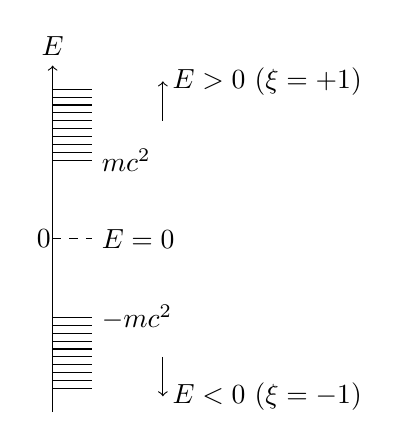
\begin{tikzpicture}[domain=-1.5:1.5]
  \draw[->] (0,-2.2) -- (0,2.2) node[above] {$E$};
  \foreach \x in {1.1, 1.2, 1.3, 1.4, 1.5, 1.6, 1.7, 1.8, 1.9}
    \draw[-] (0,\x) -- (0.5,\x) ;
  \foreach \x in {-1.1, -1.2, -1.3,-1.4, -1.5, -1.6, -1.7, -1.8, -1.9}
    \draw[-] (0,\x) -- (0.5,\x) ;
  \draw[-] (0,1) -- (0.5,1) node[right] {$mc^2$};
  \draw[-] (0,-1) -- (0.5,-1) node[right] {$-mc^2$};
  \draw[dashed] (0,0) -- (0.5,0) node[right] {$E = 0$};
  \draw[-] (0.1,0) -- (0.1, 0) node[left] {$0$};
  \draw[->] (1.4, 1.5) -- (1.4,2) node[right] {$E > 0~(\xi = +1)$};
  \draw[->] (1.4, -1.5) -- (1.4,-2) node[right] {$E < 0~(\xi = -1)$};
\end{tikzpicture}
\caption{Состояния с положительными и отрицательными энергиями.} \label{fig:14_1}
\end{figure}

$E < 0$ (отсутствуют основные состояния) - cистема неустойчива, так как электроны всегда могут перейти в состояние с меньшей энергией. (Дирак, 1930)

Чтобы устранить это противоречие, вводится понятие `моря Дирака`: все уровни с отрицательными энергиями заняты виртуальными частицами. Так как в системе электронов в одном и том же квантовом состоянии не может находиться более одного электрона, атомные электроны не могут переходить на уровни с отрицательными энергиями, система устойчива.

\begin{figure}[h!]
\centering
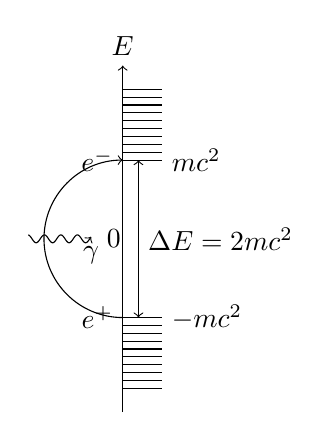
\begin{tikzpicture}[domain=-1.5:1.5]
  \draw[->] (0,-2.2) -- (0,2.2) node[above] {$E$};
  \foreach \x in {1.1, 1.2, 1.3, 1.4, 1.5, 1.6, 1.7, 1.8, 1.9}
    \draw[-] (0,\x) -- (0.5,\x) ;
  \foreach \x in {-1.1, -1.2, -1.3,-1.4, -1.5, -1.6, -1.7, -1.8, -1.9}
    \draw[-] (0,\x) -- (0.5,\x) ;
  \draw[-] (0,1) -- (0.5,1) node[right] {$mc^2$};
  \draw[-] (0,-1) -- (0.5,-1) node[right] {$-mc^2$};
  \draw[<-] (0.2,1) -- (0.2,0) node[right] {$\Delta E = 2mc^2$};
  \draw[<-] (0.2,-1) -- (0.2,0);
  \draw[-] (0.1,0) -- (0.1, 0) node[left] {$0$};
  \draw[domain=-1.2:-0.4, samples=100, ->] plot(\x, {0.05 * sin(30 * \x r) }) node [below] {$\gamma$};
  \draw [->] (0, -1) arc (-90:-270:1cm) node[left] {$e^-$};
  \node [left] at (0, -1) {$e^+$};
\end{tikzpicture}
\caption{Образование электрон-позитронной пары по действием $\gamma$-кванта. } \label{fig:14_1}
\end{figure}

$\Delta E = 2mc^2$ - порог образования электрон-позитронной пары (рис. \eqref{fig:14_1}). Она может образоваться под действием $\gamma$-кванта: электрон из `моря Дирака` перейдет в положительную энергетическую область, а на его месте образуется `дырка`. Таким образом, Дирак предсказал существование позитрона. \\

Для частицы со спином $\dfrac{1}{2}$:
$$
\Psis(\vr, t), ~~(\xi = \pm 1) \times (m_s = \pm \frac{1}{2})
$$

- 2 состояния с положительной энергией, 2 - с отрицательной. 

\begin{sloppypar}
\section{Уравнение Дирака заряженной релятивистской частицы в электромагнитном поле. Уравнение Паули}
\end{sloppypar}

$$
A^i=(\Phi, \vA)
$$

- четырехкомпонентный потенциал.

$$
H(\vr, \vp, t) = E = \sqrt{c^2\brc{\vec{p} - \frac{e}{c}\vA(\vr, t)}^2 + m^2c^4 } + e\Phi(\vr, t),
$$

где $\vec{P} = \vec{p} + \frac{e}{c}\vA(\vr, t)$.

\begin{equation}
\label{eq:14_3_1}
\boxed{i \hbar \pd{}{t} \Psis(\vr, t) = \brs{c(\aD, (\vec{p} - \frac{e}{c} \vA)) + \bD mc^2 + e\Phi} \Psis(\vr, t)}
\end{equation}

- уравнение Дирака для заряженной частицы во внешнем электромагнитном поле.

$$
\op{\vp} = - i \hbar \nabla
$$

$$
\op{\vec{p}} - \frac{e}{c} \vA \equiv \plong 
$$

- оператор удлинненного импульса. Напомним, что мы считаем заряд электрона отрицательным: $e < 0$.

Перейдем к нерелятивистскому пределу в \eqref{eq:14_3_1}:

\begin{equation}
\label{eq:14_3_2}
\Psis(\vr, t) = e^{-\frac{iEt}{\hbar}} \psi(\vr) \to \brs{E - c(\aD, \plong) - \bD mc^2 - e\Phi} \psi(\vr) = 0
\end{equation}

 В \eqref{eq:14_3_2} $\psi(\vr) = \brc{\begin{matrix} \phi(\vr) \\ \chi(\vr) \end{matrix}}$.
 
 Из \eqref{eq:14_3_2}: 
\begin{gather}
\label{eq:14_3_3}
(E - mc^2 - e\Phi) \phi(\vr) = c(\msigm, \plong) \chi(\vr) \\
(E + mc^2 - e\Phi) \chi(\vr) = c(\msigm, \plong) \phi(\vr) \nonumber
\end{gather}
 
В \eqref{eq:14_3_3} нерелятивистский предел + слабое поле.

$$
E = mc^2 + \epsilon,
$$

где $\epsilon$ - полная нерелятивистская энергия и
$$
\abs{\epsilon - e\Phi} \ll mc^2 \leftarrow \frac{\abs{\epsilon - e\Phi}}{mc^2} \sim \brc{\frac{v}{c}}^2 \ll 1
$$

Из \eqref{eq:14_3_3}

\begin{gather}
\label{eq:14_3_4}
(\epsilon - e\Phi) \phi(\vr) = c(\msigm, \plong) \chi(\vr) \\
\label{eq:14_3_5}
(2mc^2 + \epsilon - e\Phi) \chi(\vr) = c(\msigm, \plong) \phi(\vr)
\end{gather}

Из \eqref{eq:14_3_5}

\begin{equation}
\label{eq:14_3_6}
\boxed{\chi(\vr) \approx \frac{\cancel c (\msigm, \plong)}{2mc^{\cancel 2}} \phi(\vr)}
\end{equation}

$E > 0$:
$$
\underbrace{\frac{\abs{\chi(\vr)}}{\abs{\phi(\vr)}}}_{\text{`большой` или `верхний` спинор}} \sim \frac{p}{mc}  \sim \frac{v}{c} \ll 1
$$

При этом $\chi(\vr)$ - `малый` или `нижний` спинор.

Подставим \eqref{eq:14_3_6} в \eqref{eq:14_3_4}:
\begin{equation}
\label{eq:14_3_7}
(\epsilon - e\Phi)\phi(\vr) = \frac{1}{2m}(\msigm, \plong)(\msigm, \plong) \phi(\vr)
\end{equation}

\begin{excr}
Доказать, что
$$
(\msigm, \plong)(\msigm, \plong) = \plong^2 \op{1} - \frac{e\hbar}{c}(\msigm, \Hvec),
$$
где $\Hvec = rot \vA$.
\end{excr}

\begin{equation}
\label{eq:14_3_8}
\boxed{\brs{\frac{1}{2m} (\vec{p} - \frac{e}{c} \vA)^2 - \frac{e\hbar}{2mc} (\msigm, \Hvec) + e\Phi}\phi(\vr) = \epsilon \phi(\vr)}
\end{equation}

- уравнение Паули.

При этом $\frac{e\hbar}{2mc} (\msigm, \Hvec)$ описывает взаимодействие магнитного момента электрона с магнитным полем.
$$
\phi(\vr) = \brc{\begin{matrix}\phi_1 \\ \phi_2 \end{matrix}}
$$

$$
\xi = +1, \Lambda = \pm 1
$$

- спиральность. Проекция спина на направление движения. Это дает 2 спиновых состояния частицы.

$$
\xi = -1, \Lambda = \pm 1
$$

 - это дает 2 спиновых состояния античастицы.

$$
- (\mmu, \Hvec) = - \frac{e\hbar}{2mc}(\msigm, \Hvec) = \mu_B (\msigm, \Hvec), 
$$

здесь $\mu_B = -\frac{e\hbar}{2mc}$ - магнетон Бора.

\begin{equation}
\label{eq:14_3_9}
\mmu = \frac{e\hbar}{2mc} \msigm = 2 (\frac{e}{2mc})\underbrace{(\frac{\hbar\msigm}{2})}_{\op{\vec{s}}} = 2 \times \underbrace{(\frac{e}{2mc})}_{\text{гиромагнитное отношение}} \times \op{\vec{s}}
\end{equation}

Гипотеза Уленбека-Гаудсмита: магнитный момент связан с моментом частицы с $g=2$.

\section{Релятивистские поправки к уравнению Шредингера частицы во внешнем электромагнитном поле. Спин-орбитальное взаимодействие}

$$
e\Phi = U(\vr) = -\frac{e^2}{r}, ~~~\vA = 0 ~~~\Hvec = 0
$$

Из \eqref{eq:14_3_8} $\dfrac{v}{c} \ll 1$.

$$
\brs{\frac{\op{\vp}^2}{2m} + U(\vr)}\phi(\vr)=\epsilon \phi(\vr)
$$

- уравнение Шредингера.

Точность здесь $\brc{\dfrac{v}{c}}^2$.
$$
\frac{v_{\text{отн}}}{c} \sim \frac{p}{mc} \sim \frac{e^2}{\hbar c} = \alpha = \frac{1}{137}
$$

$\alpha$ - постоянная тонкой структуры.

Скорость электрона в атоме много меньше скорости света.

Из \eqref{eq:14_3_5}:
\begin{equation}
\label{eq:14_4_1}
\chi(\vr) = \frac{c(\msigm, \op{\vp})}{2mc^2 + \epsilon - e\Phi} \phi(\vr) 
\end{equation}

$$
(2mc^2 + \epsilon - e\Phi)^{-1} = \brcr{2mc^2 \brc{1 + \underbrace{\brc{\frac{\epsilon - e\Phi}{2mc^2}}}_{\sim \frac{v^2}{c^2} \ll 1}}}^{-1} = \frac{1}{2mc^2} \brc{1 - \frac{\epsilon - e\Phi}{2mc^2}}
$$

Из \eqref{eq:14_3_4} и \eqref{eq:14_4_1}:
$$
\brc{\epsilon - e\Phi}\phi(\vr) = с(\msigm, \op{\vp}) \chi(\vr) = \brcr{\frac{\cancel{c^2} (\msigm, \op{\vp})}{2m \cancel{c^2}}\brc{1 - \frac{\epsilon - e\Phi}{2mc^2}}(\msigm, \op{\vp})}
$$

Как мы знаем, $(\msigm, \vp)^2 = \op{\vp}^2$.

Тогда
\begin{equation}
\label{eq:14_4_2}
\brs{\epsilon - U(r) - \frac{\op{\vp}^2}{2m}}\phi(\vr) = - \brs{(\msigm, \op{\vp})\brc{\frac{\epsilon - U(\vr)}{4m^2c^2}}(\msigm, \op{\vp})} \phi(\vr)
\end{equation}

При этом $\bk{\phi}{\phi} \not = 1, ~~~\brc{\frac{v}{c}}^2 \ll 1$.

Теперь $\Psis = \brc{\begin{matrix} \phi \\ \chi \end{matrix}}$.

$$
1 = \int d \vr \Psis^\dag \Psis = \int d\vr (\phi^\dag \phi + \chi^\dag \chi),
$$

где $\phi^\dag = (\phi_1^*~~~\phi_2^*)$.

Из \eqref{eq:14_3_6}:
\begin{gather*}
\chi(\vr) = \frac{(\msigm, \op{\vp})}{2mc}\phi(\vr) \\
\int d\vr \brc{\phi^\dag \phi + \phi^\dag \frac{(\msigm, \op{\vp})^\dag}{2mc} \frac{(\msigm, \op{\vp})}{2mc} \phi} = 1
\end{gather*}

Заметим, что $(\msigm, \op{\vp})^\dag = (\msigm, \op{\vp})$ и $(\msigm, \op{\vp})^2 = \op{\vp}^2$.

Тогда
$$
\int d\vr \phi^\dag (\op{1} + \frac{\op{\vp}^2}{4m^2c^2}) \phi = 1  
$$

Получается, что $\bk{\phi}{\phi} \not = 1$. Но если мы будем считать, что $\bk{\phi}{\phi}= 1$, то

$$
\bfkh{\phi}{(\op{1} + \frac{\op{\vp}^2}{4m^2c^2})}{\phi} = 1  + \underbrace{\frac{v^2}{c^2}}_{\ll 1}
$$

$$
\bfkh{\phi}{(\op{1} + \frac{\op{\vp}^2}{8m^2c^2})^2}{\phi} = 1
$$
- отличие от 1 со вторым порядком малости.

Введем спинор Паули $\psi_\Pi$:
$$
\psi_\pi = \brc{\op{1} + \frac{\op{\vp}^2}{8m^2c^2}} \phi
$$

Для спинора Паули выполняется: $\bk{\psi_\Pi}{\psi_\Pi} = 1$. Можно получить, что:
\begin{equation}
\label{eq:14_4_3}
\phi = \brc{\op{1} - \frac{\op{\vp}^2}{8m^2c^2}} \psi_\Pi
\end{equation}

\begin{excr}
Используя $[\msigm \op{\vp}, f(r) \msigm \op{\vp}] = -i\hbar (\msigm, \nabla f)(\msigm, \op{\vp})$, показать, что
$$
(\msigm, \op{\vp}) U(r) (\msigm, \op{\vp}) = U(r) \op{\vp}^2 - i \hbar (\nabla U(r), \op{\vp}) + \hbar \msigm [\nabla U(r) \times \op{\vp}]
$$
\end{excr}

Подставим результат упражнения 1 в \eqref{eq:14_4_2}.

$$
\brs{\epsilon - U(r) - \frac{{\vp}^2}{2m}}\phi(\vr) = \brs{- \frac{\epsilon - U(r)}{4m^2c^2}\op{\vp}^2 + \frac{1}{4m^2 c^2} \brc{-i\hbar (\nabla U(r) \op{\vp}) + \hbar \msigm [(\nabla U) \times \op{\vp}]}} \phi(\vr)
$$

С учетом \eqref{eq:14_4_3} выразим $\phi(\vr)$:
$$
\brs{\epsilon - U(r) - \frac{{\vp}^2}{2m}}\psi_\Pi = \brs{- \frac{\epsilon - U(r)}{4m^2c^2}\op{\vp}^2 + \frac{1}{4m^2 c^2} \brc{..}} \psi_\Pi
$$

\begin{equation}
\label{eq:14_4_4}
(...) = -i\hbar (\nabla U(r), \op{\vp}) + \hbar \msigm [(\nabla U) \times \op{\vp}]
\end{equation}

$$
\nabla U(r) = \D{U}{r} \frac{\vr}{r};~~~
\hbar \msigm [(\nabla U) \times \op{\vp}] = \hbar \frac{1}{r} \D{U}{r} \msigm [\vr \times \vp] 
$$

$\vec{L} = \hbar \vec{l}$ - оператор орбитального момента частицы.

Продолжим равенство выше:
$$
\hbar \frac{1}{r} \D{U}{r} \msigm [\vr \times \vp] = {\hbar} \frac{1}{r} \D{U}{r} (\msigm, \op{\vec{L}}) = \frac{2}{r} \D{U}{r} (\op{\vec{S}}, \op{\vec{L}})
$$

Теперь правая часть \eqref{eq:14_4_4} обретает вид: 
$$\frac{1}{2m^2c^2}\frac{1}{r} \D{U}{r} (\op{\vec{S}}, \op{\vec{L}}) = \op{V_{SO}}$$

- оператор спин-орбитального взаимодействия.

В поле ядра:

\begin{gather*}
U(r) = -\frac{Ze^2}{r} \\
\boxed{A_{S0} (r) = \frac{Ze^2 \hbar^2}{2m^2 c^2 r^3} > 0}
\end{gather*}

Природа спин-орбитального взаимодействия. Рассмотрим электрон.

$$
\mu = \frac{e}{mc}\hbar \op{\vec{s}}
$$

\begin{figure}[h!]
\centering
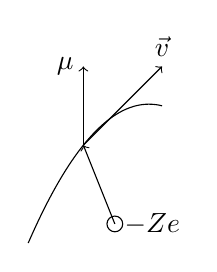
\begin{tikzpicture}[domain=-2:2]
  \draw[->] (0, 0) -- (1, 1) node[above] {$\vec{v}$};
  \draw[->] (0, 0) -- (0,1) node[left] {$\bm{\mu}$};
  \draw[<-] (0, 0) -- (0.4,-1) node[right] {$-Ze$};
  \draw[domain=-0.7:1, samples=50] plot(\x,{-0.75 * \x * \x + 1.25 * \x});
  \draw (0.4, -1) circle (1mm); 
\end{tikzpicture}
\caption{К вопросу о спин-орбитальном взаимодействии.} \label{fig:14_3}
\end{figure}


$$
\vec{L} = m[\vr \times \vec{v}]
$$

$$
\vec{E} = - \nabla \Phi(r) = -\D{\Phi}{r} \frac{\vr}{r}
$$

(см. Теорию поля)

$$
\Hvec = \frac{1}{c}[\vec{E} \times \vec{v}]
$$

$$
\op{V_m} = - \mu \Hvec = \brc{-\frac{e\hbar}{mc}} \frac{1}{r}\brc{-\frac{1}{c} \D{\Phi}{r}}\brc{\op{\vec{s}} [\vp \times \vec{v}]} = \underbrace{\frac{\hbar^2}{m^2c^2} \frac{1}{r} \D{U(r)}{r} (\vec{s}, \vec{l})}_{}
$$

Спин-орбитальное взаимодействие можно трактовать, как взаимодействие спина с магнитным полем ядра (рис. \eqref{fig:14_3}).

\begin{excr}
Доказать, что в пределах требуемой точности $\brc{\frac{v}{c}}^2$: 
$$
(\epsilon - U(r)) \op{\vp}^2 = \frac{\op{\vp}^4}{2m} - \hbar^2 \Delta U(r) - 2i\hbar(\nabla U(r), \op{\vp})
$$
\end{excr}

Подставим результат упражнения 2 в \eqref{eq:14_4_4}:

\begin{gather*}
\brs{\epsilon - U(r) - \frac{{\vp}^2}{2m}}\psi_\Pi = \brs{ -\frac{\op{\vp}^4}{8m^3c^2} + \frac{1}{8} \brc{\frac{\hbar}{mc}}^2 \Delta U(r) + \op{V_{SO}}} \psi_\Pi
\end{gather*}

или

$$
\brs{\epsilon - U(r) - \frac{{\vp}^2}{2m}}\psi_\Pi = \op{V_{\text{кв. рел.}}} \psi_\Pi
$$

где

\begin{equation}
\label{eq:14_4_5}
\op{V_{\text{кв. рел.}}} = \op{V_1} + \op{V_2} + \op{V_{SO}}
\end{equation}

$\brc{\frac{v}{c}}^2$ - квазирелятивистское приближение.

$V_1 = -\frac{\op{\vp}^4}{8m^3c^2}$ - релятивистская поправка к параметру потенциальной энергии.

$
K = \sqrt{m^2c^4 + c^2p^2} - mc^2 = mc^2\brc{1 + \frac{\op{\vp}^2}{m^2c^2}}^{1/2} - mc^2 \approx mc^2\brc{1 + \frac{\op{\vp}^2}{2m^2c^2} - \frac{\op{\vp}^4}{8m^2c^4}} - mc^2 = \frac{\op{\vp}^2}{2m} - \frac{\op{\vp}^4}{8m^3c^2}
$

$$
\op{V_2} = \frac{1}{8} \brc{\frac{\hbar}{mc}}^2\Delta U(r) 
$$

- оператор контактного взаимодействия электрона с ядром

$$
U(r)  = -\frac{Ze^2}{r} \to \Delta U(r) = -Ze^2 \Delta \brc{\frac{1}{r}} = 4 \pi Ze^2 \delta(\vr)
$$

$$
\op{V_2} = \frac{\pi}{2} \brc{\frac{\hbar}{mc}}^2 Ze^2 \delta(\vr) \to \avg{\op{V_2}} \not = 0, ~\vr = 0
$$

Таким образом, получаем:
$$
\avg{\op{V_2}} \sim \abs{\psi(0)}^2 \not = 0
$$

Вспомним, что $R_{nl}(r) \sim r^l$, $l=0$, т.е. для s-состояний: 
$\avg{\op{V_{SO}}}$ и $\avg{(\op{\vec{s}}, \op{\vec{l}})} \neq 0$ при $l \neq 0$.
